\documentclass{article}%
\usepackage[T1]{fontenc}%
\usepackage[utf8]{inputenc}%
\usepackage{lmodern}%
\usepackage{textcomp}%
\usepackage{lastpage}%
\usepackage{authblk}%
\usepackage{graphicx}%
%
\title{Kaiso is expressed in lung cancer: Its expression and localization is affected by p120ctn}%
\author{Justin Scott}%
\affil{Departments of Medicine, Biochemistry and Molecular Biology, Indiana University School of Medicine, The Melvin and Bren Simon Cancer Center and the Center for Pancreatic Cancer Research, Indianapolis, Indiana, United States of America}%
\date{01{-}01{-}2013}%
%
\begin{document}%
\normalsize%
\maketitle%
\section{Abstract}%
\label{sec:Abstract}%
SAN DIEGO {-} According to health officials, Integrated System{-}Rometers (ISDs) have been released into the waters of the Atlantic from California and Florida (in addition to Miami, Florida).\newline%
The strategy will allow for both colony and infective strains of the organism to survive the isolation and ultimately eradicate the entire organism and destroy the surrounding environment.\newline%
Newcastle University pathology professor Brian Harrigan provided 10News with this insight regarding the ISDs strategy and possible strategy of elimination, oral administration and albumin suppression methods.\newline%
The operation will be conducted along the Linesque River and Robert Trent Jones Drive in San Diego County. The ISDs are commonly used in solid processing of sensitive pathogens in human and animal wounds, especially C difficile.\newline%
Interim packages of ISDs are subject to special seals, and are odor{-} and fragrance{-}free. As a protective method, the paste is mixed into fish or other unpublicized neutralization products.\newline%
How peri{-}infective is ISD isolated and treated?\newline%
The bacterium is isolated and treated based on symptoms or pathology of the organism. Depending on the conditions and the severity of infection, these products can be added to raw meat, seafood or other products.\newline%
For example, the ISDs are infused into wounds or other tissue and treated with antibiotics.\newline%
Alternatively, a manner may be required based on the symptoms that cause an infection. An infection may be treated with the ISDs or a bacterial killer such as vincristine. If infection is mild or life{-}threatening, ISDs can be removed from the wounds using auto injection.\newline%
Does it necessarily need to be eliminated in animal and human infection in order to be effective?\newline%
It would take a very strict use of the ISDs and the pH (according to temperature) setting of the organism.\newline%
If this becomes necessary then ISDs can be used to decontaminate or remove animal and human infections in animal and human wounds.

%
\subsection{Image Analysis}%
\label{subsec:ImageAnalysis}%


\begin{figure}[h!]%
\centering%
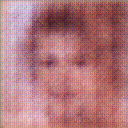
\includegraphics[width=150px]{500_fake_images/samples_5_165.png}%
\caption{A Close Up Of A Person Wearing A Tie}%
\end{figure}

%
\end{document}